 \chapter{Методика исследования}

 \section{Использование информации о фактическом времени ответа}

Выражение для прогнозного времени ответа можно использовать для вы\-явления абер\-раций (отклонений) в поведении пользователя. Для этого введём понятие отклонения прогноза.

Отклонением прогноза будем разность между прогнозным временем ответа и фактичес\-ким временем ответа студента. В логарифмической шкале разность будет иметь вид отноше\-ния
\begin{equation}
E_{ij} = \ln \tilde{T}_{ij} - \ln t_{ij} =  \ln \frac{\tilde{T}_{ij}}{t_{ij}}
\end{equation}

Из этого отношения можно сделать вывод, что ошибка прогноза - случайная величина, которая имеет нормальное распределение c параметрами
\begin{equation}
E_{ij} \sim N\left(\mu + \beta_i + \tau_j - \ln t_{ij},\frac{n\sigma^2}{k-1}\right).
\end{equation}

Таким образом, выявление отклонений в поведении студента сводится к задаче проверки статистической гипотезы о том, что реализации $e_{ij}$ случайной величины $E_{ij}$ имеют нормаль\-ное распределение против альтернативы, что ошибка прогноза имеет какое-либо другое распреде\-ление
$$
\begin{array}{lll}
H_0 &:& e_{ij} \sim N\left(\mu + \beta_i + \tau_j - \ln t_{ij},\frac{k\sigma^2}{k-1}\right)\\
H_1 &:& \mbox{ошибка прогноза имеет другое распределение}
\end{array}
$$

\section{Обработка экспериментальных данных}

\subsection{Источник экспериментальных данных}

Для применения на практике теоретических положений и математических моделей, описанных в Главе \ref{ch22} использовались реальные данные пользователей системы дистанцион\-ного обучения МАИ. На момент написания диплома в системе не фиксировалось время, которое студент тратит на решение конт\-рольных и тестовых задач. В связи с этим в исходный код системы дистан\-ционного обучения и структуру базы данных, которая исполь\-зуется системой дистанционного обучения, были внесены доработки, позволяющие фикси\-ровать время ответа для всех существующих курсов (<<Математический ана\-лиз>>, <<Линейная алгебра и аналитическая геометрия>>, <<Теория вероятностей и математическая статистика>>).

После внесённых изменений система фиксирует следующие данные: сколь\-ко раз была отображена каждая задача, сколько попыток произвел каждый студент для её решения, какое количество времени было затрачено для каждой из попыток и насколько удачной была попытка (верно или неверно решена задача)

\subsection{Оценка параметров по выборке}

\subsubsection{Преобработка полученных данных}

Для получения оценок параметров модели, описанных в разделе \ref{opm}, обработаем полученную статистику. Порядок обработки статистики покажем на примере задачи № 8.2.3 из курса <<Математический анализ>>

\newpage
Вначале построим гистограмму для времени, которое студенты затра\-чивали для ответа на задачу
\begin{figure}[ht!]
\centering 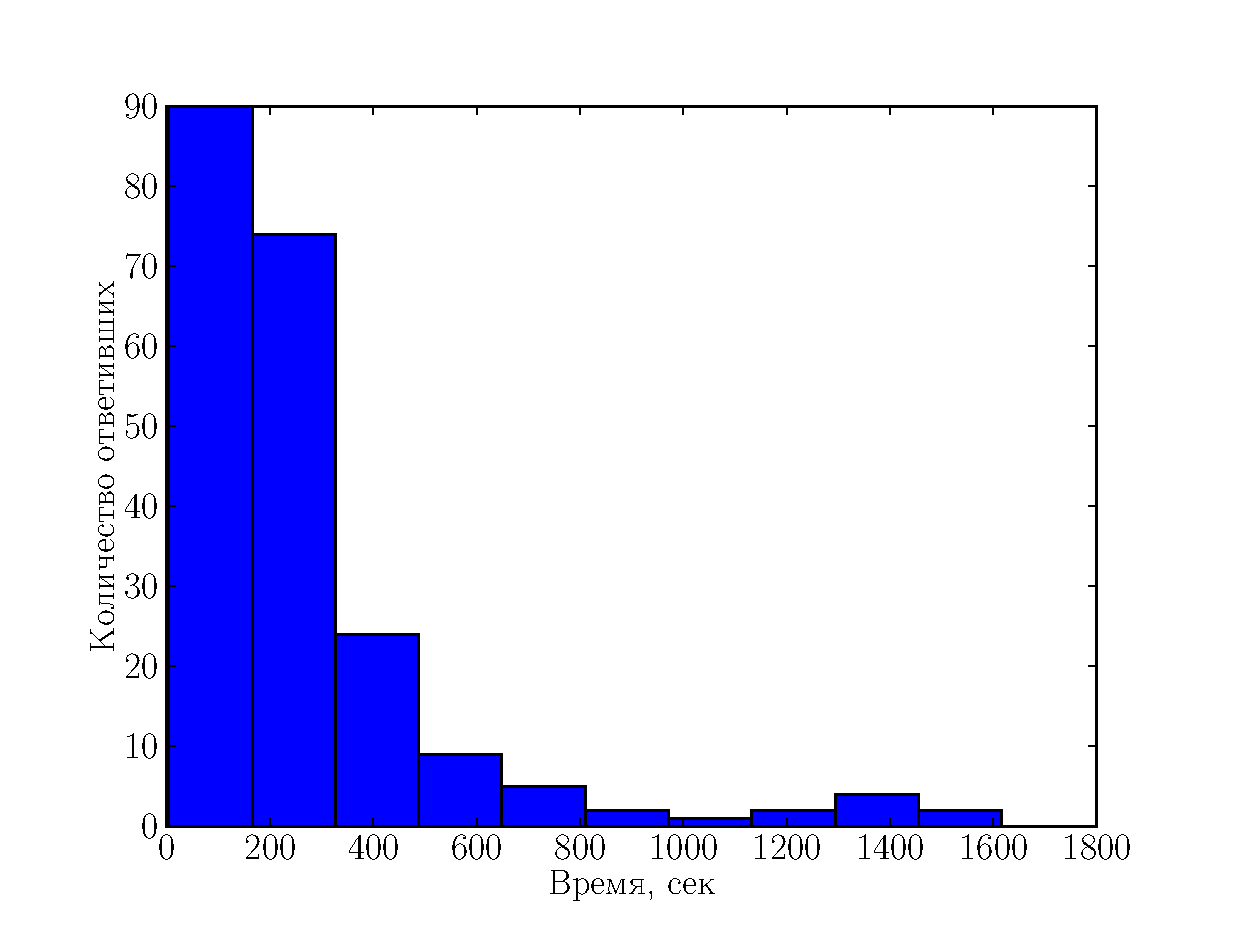
\includegraphics[scale=0.6]{test.eps}
\caption{Гистограмма времени ответа}
\end{figure}

Согласно модели, построенной в разделе (\ref{mvonu}), применим логарифми\-ческое преобразование к времени ответа и построим гистограмму полученных значений:
\begin{figure}[ht!]
\centering 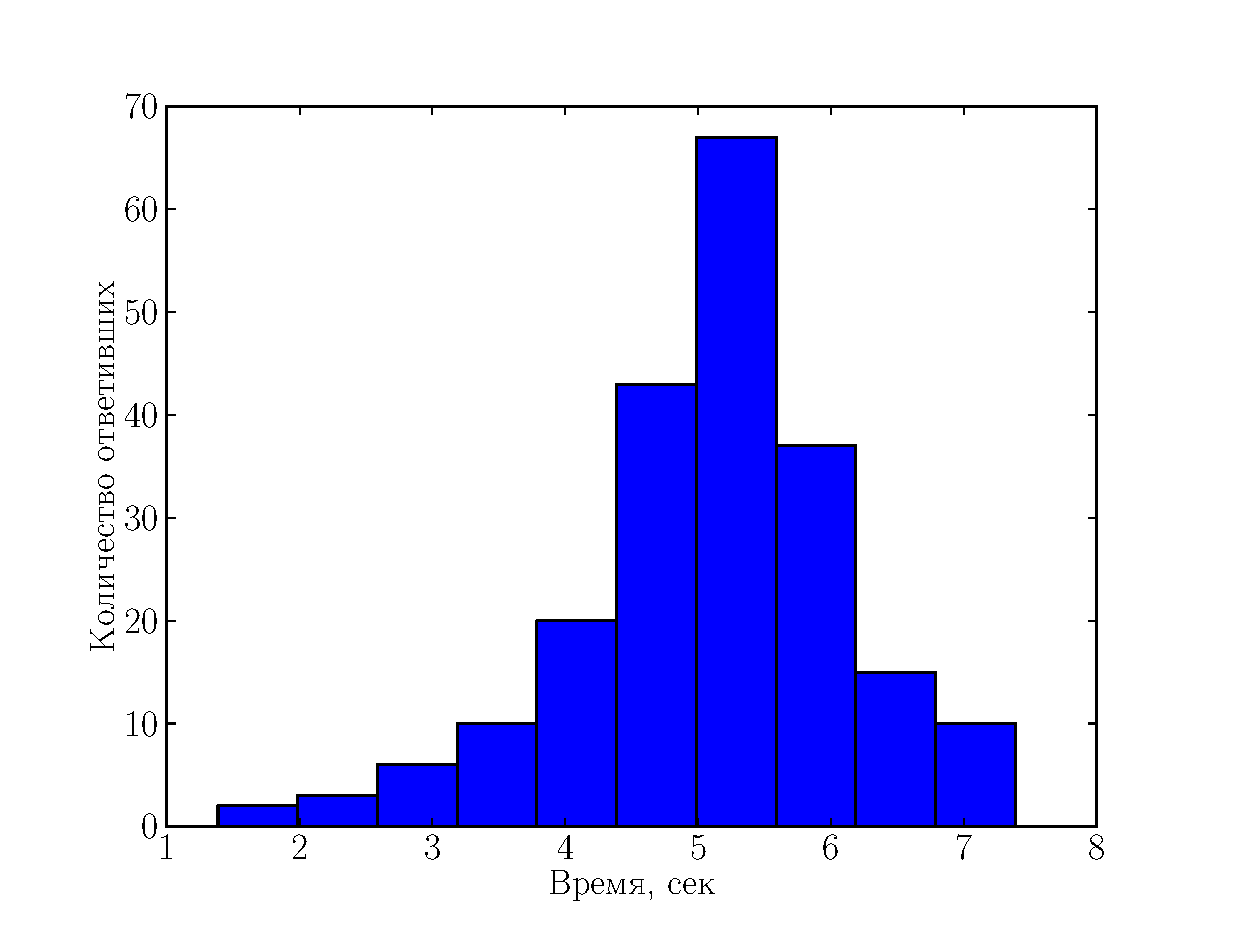
\includegraphics[scale=0.6]{test1.eps}
\caption{Гистограмма времени ответа (логарифмический масштаб)}
\end{figure}

Как видно из данного примера, прменение логарифмического преобра\-зования к выборке по времени ответа обучающихся на конкретную задачу в системе дистанционного обучения позволяет получить симметричный вид распределения, который походит на гауссовское распределение. Проверка на гауссовость приводится в следующих разделах.

\subsubsection{Оценка параметров модели}

Модель, описанная уравнением (\ref{predictedtime}) в применении к экспериментальным данным имеет следующий вид. Пусть, согласно пункту (\ref{opm}) для каждого студента $j$ из общего количества студентов $M$ система дистанционного обучения случайным образом выбирает $k$ задач из пула задач объёма $K$. Тогда по результатам тестирования мы получаем следующую таблицу:
\begin{table}[H]
\caption{Время ответа}
\label{tabular:IRTtable}
\begin{center}
\begin{tabular}{|c|c|c|c|c|}
\hline
 & \multicolumn{4}{|c|}{Задача}\\
 \hline
 Студент & 1 & 2 & \dots & k \\
 \hline
 1 & $t_{11}$ & $t_{12}$ & \dots & $t_{1k}$\\
\hline
 2 & $t_{21}$ & $t_{22}$ & \dots & $t_{2k}$\\
\hline
 \vdots & \vdots & \vdots & \vdots & \vdots\\
\hline
 M & $t_{M1}$ & $t_{M2}$ & \dots & $t_{Mk}$\\
\hline
\end{tabular}
\end{center}
\end{table}

Таблица отражает время $t_{ij}$, которое затратил студент  $j$ при ответе на задачу $i$. Время ответа имеет логнормальное распределение, согласно п. (\ref{mainmodel}).

Оценка параметров модели происходит на основании данных таблицы (\ref{tabular:IRTtable}) согласно формулам (\ref{1166}) - (\ref{1167}).

\subsection{Проверка предположения о гауссовости}

Проверим гипотезу о гауссовом распределении времени ответа студента. Для этого сформулируем основную и альтернативную гипотезы следующего вида:
$$
\begin{array}{lll}
H_0 &:& t_{ij} \sim N\left(\mu,\sigma^2\right)\\
H_1 &:& t_{ij} \mbox{ имеет другое распределение}
\end{array}
$$

\subsection{Применение модели}

Используя оценки, полученные в пункте \ref{opmpv}, продемонстрируем работу модели для выявления отклонений в поведении студентов.

\subsubsection{Моделирование данных}

Для оценки параметров модели воспользуемся базой данных системы дис\-танционного обучения МАИ по курсу <<Математический анализ>>.

В тестировании принимало участие $30$ обучающихся. Система дистанционного обучения предлагает каждому студенту $k=16$ задач.

%Запрос для кол-ва пользователей select count(distinct user) from matan_www_irt where item='7.3.6';

Cогласно формулам (\ref{1166}) - (\ref{1167}) были получены оценки параметров модели $\tau_j$ (для каждого студента), $\beta_j$ (для каждой задачи) и $\mu$ (временной параметр, обобщающий все полученные данные).

Для проверки работы модели смоделируем две последовательности - после\-довательность значений времени ответа на задачи теста для студента, который отвечает на задачи теста <<честно>> и аналогичную последовательность для студента, который пользуется готовыми ответами на некоторые задачи.

Для моделирования <<мошеннических>> ответов воспользуемся следующим приёмом, описанным в \cite{6.}. Согласно формуле (\ref{mainmodel}), время ответа студента, который не обладает ответами на задачи, имеет логнормальное распределение:
$$
\ln T_{ij} \sim N (\mu + \beta_i + \tau_j, \sigma^2),
$$
а если студент $j$ получил ответ на задачу $i$ заранее, то время ответа так же имеет логнормальное распределение, но с другим параметром смещения:
$$
\ln T_{ij} \sim N (\mu + \beta_i + \tau_j + L, \sigma^2),
$$
где $L$ - параметр смещения, который задаётся исследователем. В \cite{6.} в качестве значения $L$ принимается оценка дисперсии параметра $\tau_j$, взятая с противо\-положным знаком:
\begin{equation}
\label{fraudlevel}
L = (-1)\cdot Var\left( \hat{\tau_j}\right) = (-1)\cdot \frac{\sigma^2}{k}
\end{equation}

Выберем из группы студента случайным образом. Пусть у выбранного студента имеются заранее подготовленные ответы на задачи под номерами $[5,9,15]$. Проведём моделирование ответов студента, который <<мошенничает>> при прохождении теста, параметр смещения определим из соотношения (\ref{fraudlevel}).

Так же для этого студента рассчитаем прогнозное время ответа. На стол\-бчатой диаграмме отобразим прогнозное и смоделированное время ответа. Для наглядности прогнозное время ответа отображается <<как есть>>, а вместо значения смоделированной величины берём ей противоположную . Над каж\-дым столбцом подписано соответствующее ему числовое значение (для удоб\-ства).

\begin{figure}[ht!]
\centering 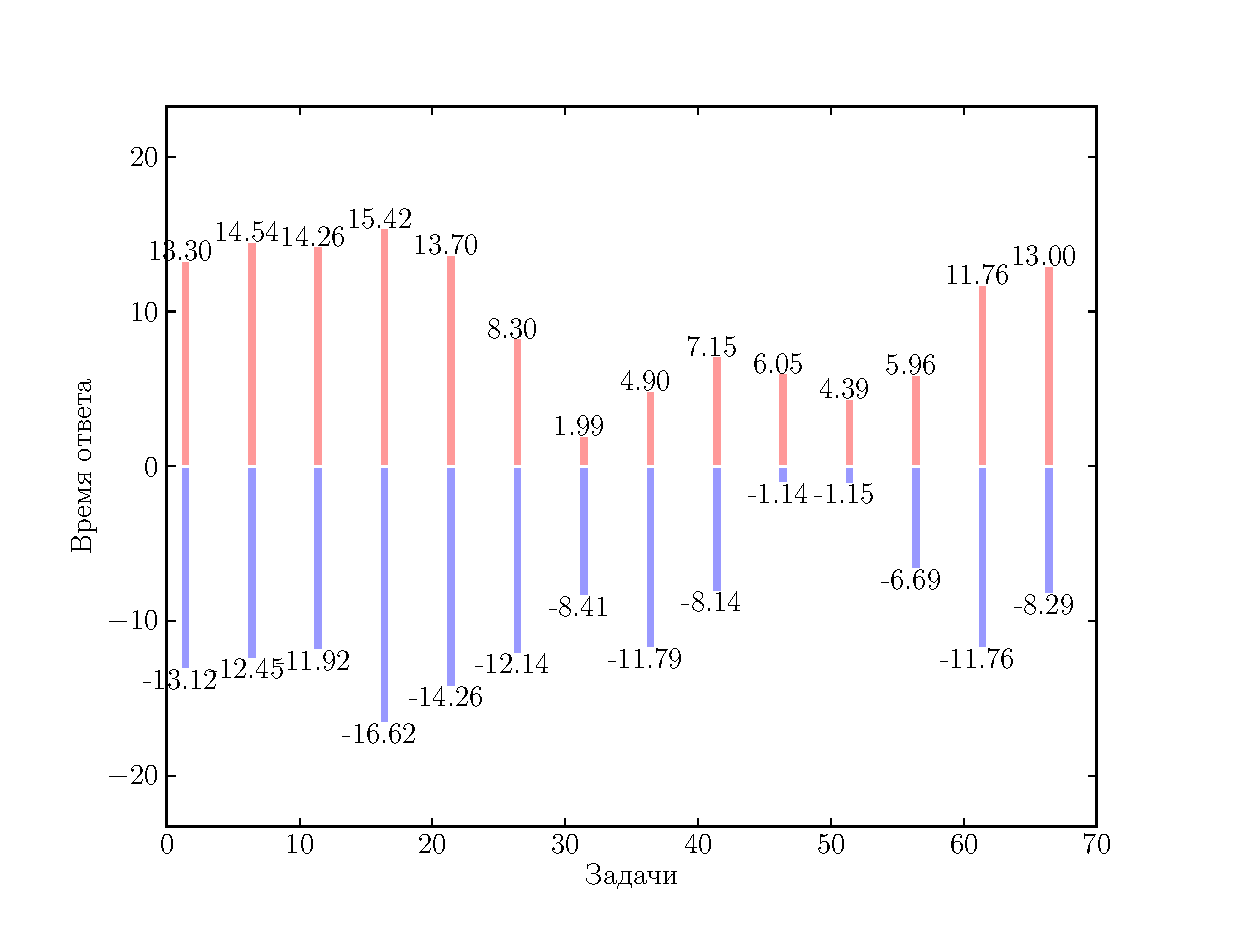
\includegraphics[scale=0.85]{forecast.eps}
\caption{Сравнение прогнозных и модельных данных}
\end{figure}